\documentclass[12pt]{article}

\setlength{\oddsidemargin}{-0.25 in}
\setlength{\evensidemargin}{-0.25 in}
\setlength{\topmargin}{-0.9 in}
\setlength{\textwidth}{7.0 in}
\setlength{\textheight}{9.0 in}
\setlength{\headsep}{0.75 in}
\setlength{\parindent}{0.0 in}
\setlength{\parskip}{0.0 in}

\usepackage{graphicx}
\usepackage{wrapfig}
\usepackage{color}
\usepackage{caption}
\usepackage{subcaption}
\usepackage{amsmath}
\usepackage{multirow}

\captionsetup{justification=centering}

\begin{document}
\begin{center}
Analysis of Heuristics for the Number Partition Problem \\
George Zhang \\
CS124 Programming Assignment 3 Writeup \\
https://github.com/gzhang01/cs124prog/tree/master/prog3 \\
\end{center}

\section{Abstract}
Our goal was to implement heuristics for solving the number partition problem. We started with the deterministic Karmarkar-Karp (KK) algorithm and then moved to several randomized heuristics, including repeated random (RR), hill climbing (HC), and simulated annealing (SA). For each of the randomized algorithms, we looked at the results with two representations of the solution: as a sequence (S) of $\{-1, +1\}$ values determining the sets and as a prepartitioning (P) of the numbers. We found that the P representation produced much better results than the S representation (about a million-fold final residue improvement), though it also took about 100 times longer to run. In addition, SA performed significantly better than HC and mildly better than RR.

\section{Introduction}
The number partition problem can be stated as follows: given an input $A = (a_1, a_2, \dots, a_n)$ of non-negative integers, produce a sequence $S = (s_1, s_2, \dots, s_n)$ of signs $s_i \in \{-1, +1\}$ such that the residue
$$u = \left| \sum_{i = 1}^n s_ia_i \right|$$
is minimized. Analogously, we are trying to split the integers in $A$ into two sets $A_1$ and $A_2$ such that the sums of $A_1$ and $A_2$ are as similar as possible, with the residue being the absolute value of the difference between the sets. Even though this problem is NP-complete, there does exist a pseudo-polynomial time dynamic programming algorithm for it. \\

\textbf{Dynamic Programming Solution} \\
To start, instead of considering the optimization problem, let us consider the yes/no problem as follows: given an input $A$, is there a way to partition $A$ into $A_1$ and $A_2$ such that the sums of $A_1$ and $A_2$ are equal? We let $b$ be the sum of the sum of the elements in $A$, and so our question becomes whether we can produce a set $A_1$ such that the sum of the elements in $A_1$ is equal to $\lfloor b/2 \rfloor$. Note that if $b$ is odd, the sum of $A_2$ will be $\lceil b/2 \rceil$, but we shall for our purposes say that this off by one answer still produces a "yes" result to our question. We shall see that with the filled array from this question, we can produce the answer to the optimization problem. \\

To obtain the answer to this question, we shall let $D(i, k)$ represent whether there exists a subset of $(a_1, \dots a_i)$ whose elements sum to $k$. The answer we want, then, is the value $D(n, \lfloor b/2 \rfloor)$. We notice that all sets have a subset whose elements sum to zero: namely the empty subset. We also notice that in order for a set $(a_1, \dots, a_i)$ to contain a subset whose elements sum to $k$, either the set $(a_1, \dots, a_{i - 1})$ contains a subset whose elements sum to $k$, or that set contains a subset whose elements sum to $k - a_i$. Thus mathematically, we have: \\
$$D(i, 0) = \text{True}$$
$$D(i, k) = D(i - 1, k) \text{ or } D(i - 1, k - a_i)$$

Using this recurrence, we fill an array of size $n \times \lfloor b/2 \rfloor$. Our answer is the value $D(n, \lfloor b/2 \rfloor)$. We notice that each square in the array takes constant time to fill, since we are accessing two values in the array, and we iterate over the entire array. Thus the run time of this algorithm will be $O(nb)$, and correctness follows from the logic of the recurrence. \\

However, this does not yet give us an answer to the optimization problem we want to solve. We notice that if $D(n, \lfloor b/2 \rfloor)$ is True, then we know the optimal residue: $0$ if $b$ is even and $1$ if $b$ is odd. If $D(n, \lfloor b/2 \rfloor)$ is False, then we can look at $D(n, \lfloor b/2 \rfloor - 1)$. If this is True, then we know that the optimal residue must be $2$ if $b$ is even and $3$ if $b$ is odd, since if one set sums to $\lfloor b/2 \rfloor - 1$, the other set must sum to $\lceil b/2 \rceil + 1$, and the difference between the sum of sets is either $2$ or $3$ depending on the parity of $b$. This pattern continues, and thus we have an algorithm for finding the solution to the optimization problem based on our existing array: find the smallest $p \ge 0$ such that $D(n, \lfloor b/2 \rfloor - p)$ is True. The smallest residue is the $2p$ if $b$ is even and $2p+1$ if $b$ is odd. The final step at worst travels up one dimension of the array, and so it has runtime $O(b)$, and thus the solution to the optimization problem is still $O(nb)$, or pseudo-polynomial time. \\

\textbf{Karmarkar-Karp Algorithm} \\
The Karmarkar-Karp algorithm is a deterministic heuristic for the Number Partition problem. It repeatedly takes the two largest numbers in $A$ and replaces them with their difference, with the intuition being that placing the two numbers in different sets is analogous to placing their difference in some set. \\

If we assume that arithmetic operations take constant time, we can implement the KK algorithm in $O(n \log n)$ time using a max heap. Initialization of the heap will take about $O(n \log n)$ time, since insertion is $O(\log n)$ and there are $n$ elements to insert (of course, this is a loose bound, since insertion will really only take log of the number of elements already in the heap). Each step in KK will require popping two elements off the heap and inserting back on. Each of these actions require $O(\log n)$ time, so the total for a single step is still $O(\log n)$, since we are doing a constant number of these actions. Finally, we run the algorithm for $n - 1$ steps to remove all but one element, and so the entire algorithm runs in $O(n \log n)$ time with a max heap. \\

\textbf{Representations of Solutions and Other Heuristics} \\
There are two representations of solutions we will consider. One is simply a set $S$ of $+1$ and $-1$ values. We create a random solution by choosing $n$ values from $\{-1, +1\}$, and we define a move from one solution to another as changing a random element's set $s_i$ to $-s_i$, and with probability $1/2$ changing another random element's set from $s_j$ to $-s_j$. We can also represent our solution via prepartitioning, Here a solution is of the form $P = \{p_1, \dots, p_n\}$ where $p_i \in \{1, \cdots, n\}$ and if $p_i = p_j$, then $a_i, a_j$ are in the same set. A random solution in this representation will assign values from $1$ to $n$ for all the $p_i$ and then run KK on the prepartition to produce the two subsets. We define a move on this state space by selecting a $p_i$ and assigning it a different value on $[1, n]$. \\

There are also three other heuristics to consider. The first is repeated random, where we repeated generate random solutions to the problem and keep the best one (where "best" is defined as the one with the lowest residue). The second is hill climbing, where we start with a random solution and then try to improve it through moves to better neighbors. Finally, we will consider simulated annealing, where we'll generate a random solution and then try to improve it by moving to neighbors which may not always be better -- that is we will always move to a neighbor that is better, but we will move to a neighbor that is not better with some probability $P$ that may be a function of how long our algorithm has run. \\

Our goal will be to implement the KK algorithm, as well as our three other heuristics each using both representations. We will then compare the success of these heuristics as well as their running times.

\section{Implementation}
We began by first implementing the Karmarkar-Karp algorithm. To maintain the $O(n \log n)$ runtime, we decided to implement a max-heap data structure (see heap.c). When that was completed, implementing KK was very straightforward, as we would simply insert all the numbers into the max-heap and pop two numbers and insert their difference at each step until there was only one number remaining (see function kk in main.c). \\

We then moved on to writing some functions that generated random solutions and found random neighbors with both representations (see solution.c). These were fairly straightforward with the given descriptions in the spec. We decided that we would seed our random number generator whenever someone called the function to generate a solution. Even though we needed to produce random numbers when finding neighbors, we decided it was safe to assume that a particular solution was generated first before any neighbors had to be generated. \\

The final step was to implement the heuristics. To do this, we started by writing functions to compute the residue of a given solution based on the solution type. The heuristics themselves were slightly repetitive, as most followed the same structure, but had different conditions on when values would be updated. Both here and during implementation of random solution generators, we decided that an object-oriented language would have made things much simpler. Since both the sequence and partition representations were solutions, it would have made sense to have a solution class, which sequence and partition would inherit from. Sequence and partition could then overwrite functions to generate solution, find random neighbors, and find residues to fit their specific requirements. Calling these functions would be simple in this case, since they would have the same name, and their implementations would depend on what type it was. Given that C is not an object oriented language, we had to make do with conditions that identified whether we had a sequence or partition and call the correct function (see mess of functions in main.c). \\

After the implementation was done, we wrote a few more lines that implemented the behavior expected by the spec with regards to input files and output. We also wrote a few functions that returned residues for each of the methods so we could more easily discuss our results. 

\section{Results}
in order to compare the results, we ran 50 test trials on randomly generated numbers on the range $[1, 10^{12}]$. For each test trial, we produced the residue given by the KK algorithm, the initial residues of the randomly chosen start solution, and the final residues of each of the heuristics. In order to better compare results within a trial, we started with the same random start solution for each of the heuristics within a single trial (of course, we chose new start solutions on different trials). Because sequence and partition represent their solutions differently, we produced both a sequence random solution and a partition random solution to begin with. The complete data for all 50 trials are in appendix A. Below are the average residues over the 50 trials. KK results are shown first, followed by initial residue, final repeated random, final hill climbing, and final simulated annealing for sequence-based solutions, and finally the same four for partition-based solutions.

\begin{table}[h]
\renewcommand{\arraystretch}{1.3}
\begin{center}
\begin{tabular}{c | c c c c | c c c c}
\multirow{2}{*}{KK} & \multicolumn{4}{c|}{Sequence} & \multicolumn{4}{c}{Partition} \\
& R & RR & HC & SA & R & RR & HC & SA \\ \hline
292029 & 4255641605057 & 252865950 & 353262590 & 248113800 & 9610309 & 240 & 711 & 212 \\
\end{tabular}
\caption{Average Residues for Various Heuristics}
\end{center}
\end{table}

We were also interested in which heuristic performed the best given any particular trial. The table below shows the various heuristics and the number of 1st, 2nd, and last place rankings with regard to the final residue:

\begin{table}[h]
\setlength{\tabcolsep}{20pt}
\begin{center}
\begin{tabular}{c | c c c | c c c}
\multirow{2}{*}{Place} & \multicolumn{3}{c|}{Sequence} & \multicolumn{3}{c}{Partition} \\
& RR & HC & SA & RR & HC & SA \\ \hline
1st & 19 & 16 & 15 & 18 & 8 & 24 \\
2nd & 14 & 15 & 21 & 21 & 14 & 15 \\
3rd & 17 & 19 & 14 & 11 & 28 & 11 \\
\end{tabular}
\caption{Frequency of Rankings Among Heuristics}
\end{center}
\end{table}

We also looked at the run times of each of the heuristics. The complete data for all 50 trials are in appendix B. Below are the average runtimes over the 50 trials. Data for repeated random, hill climbing, and simulated annealing are shown for sequence and partition-based data. Note that times shown are in milliseconds.

\begin{table}[h]
\renewcommand{\arraystretch}{1.3}
\setlength{\tabcolsep}{20pt}
\begin{center}
\begin{tabular}{c c c | c c c}
\multicolumn{3}{c|}{Sequence} & \multicolumn{3}{c}{Partition} \\
RR & HC & SA & RR & HC & SA \\ \hline
37 & 18 & 19 & 1654 & 1551 & 1544 \\
\end{tabular}
\caption{Average Runtimes for Various Heuristics}
\end{center}
\end{table}

While average values and rankings are good, we also want to see trends in the full data. Below are scatter plots showing results from all 50 trials. Note that the dots are color-coded based on KK (red), sequence solutions (blue), and prepartition solutions (green), and the y-axis in both graphs are on a logarithm scale. The runtimes graph only lists runtimes for the randomized algorithms, as the time to run KK or find initial residues is negligible.

\begin{figure}[h]
\begin{subfigure}[t]{0.5\textwidth}
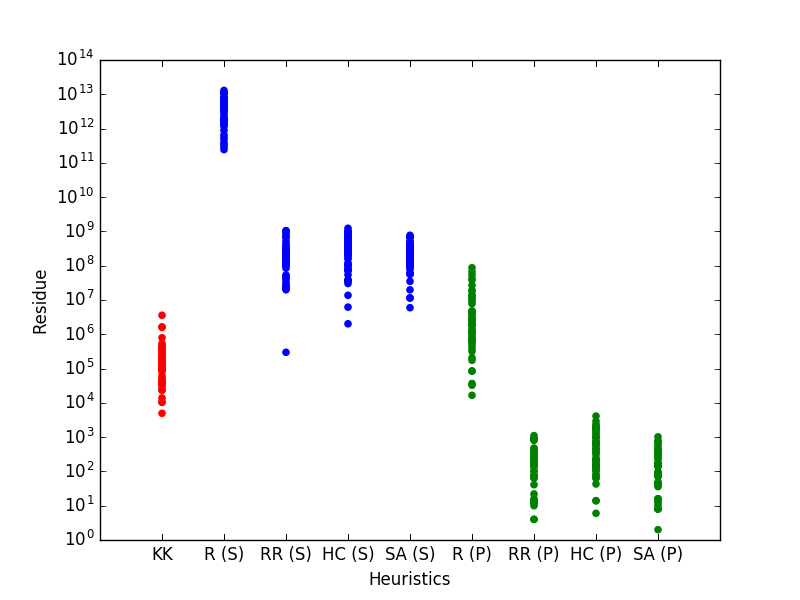
\includegraphics[width=\textwidth]{img/residues.png}
\caption{Residue Values}
\end{subfigure}
\begin{subfigure}[t]{0.5\textwidth}
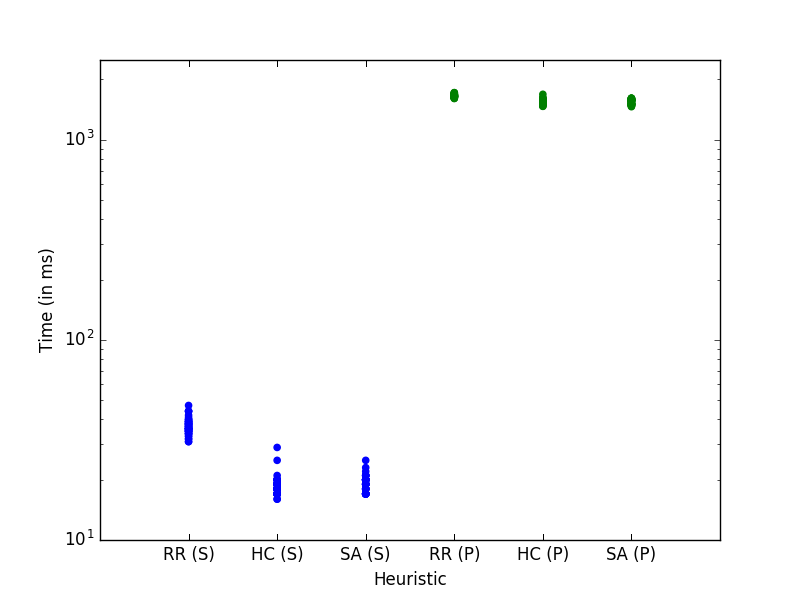
\includegraphics[width=\textwidth]{img/times.png}
\caption{Runtimes}
\end{subfigure}
\caption{Heuristic Data}
\end{figure}

As we can see from the tables and the graphs, prepartition-based solutions produce better results than sequence-based solutions. Even without running any randomized algorithms, the initial residue found from a completely randomly chosen solution is better for the prepartition case than for the sequence case. This result makes sense, since the sequence solution uniquely places each number into a set, whereas the prepartition solution merely groups a few numbers together and then runs KK on the resulting set. Thus there is much more flexibility in the prepartition case than the sequence case, and so we see a lower residue. Indeed, judging from the averages, prepartitioning produces final residues that are on the order of one-million times better than the sequence residues. \\

However, this flexibility and lower residue values comes at the cost of computing time. Since prepartitioning assigns groups to the numbers and does not produce a solution by itself, it must run the KK algorithm to find the residue. This is more costly than simply summing the values based on subset that we could do with a sequence solution, and so we would expect a higher runtime. This is indeed the case, as we can see in graph b. on average, prepartitioning increases the runtime of the algorithms by 100 times as compared to the sequence runtimes. \\

We also want to look at the heuristics themselves. From the data, we can see that hill climbing generally produced the worst residues on average among both sequence and prepartition solutions. However, the rankings of heuristics given trial is a bit more mixed for the sequence solutions than the prepartition solutions. We can see that each of the three heuristics had similar numbers of trials where they performed the best given sequence solutions. The prepartition solutions, however, generally followed a trend of SA being the best, followed by RR and then HC. The graphical data also supports this, as the data for sequence solutions are closer together than the data for prepartition solutions, suggesting a bit more variance in which solution performed best. Based on the averages, though, we can conclude that SA did better than the HC, which makes sense since HC is susceptible to getting stuck at local optima. \\

To really look at how these heuristics compare, we also collected data on residue values while the program is running. We logged the residue value of the random solution / neighbor as well as the best reside for each of the 25000 iterations (for the SA case, we also logged the neighbor we are currently on, which may not be the best one). The data is shown below, where green is best residue value, blue is random residue value, and in the case of SA, red is current neighbor residue:

\begin{figure}[h]
\begin{center}
\begin{subfigure}[t]{0.3\textwidth}
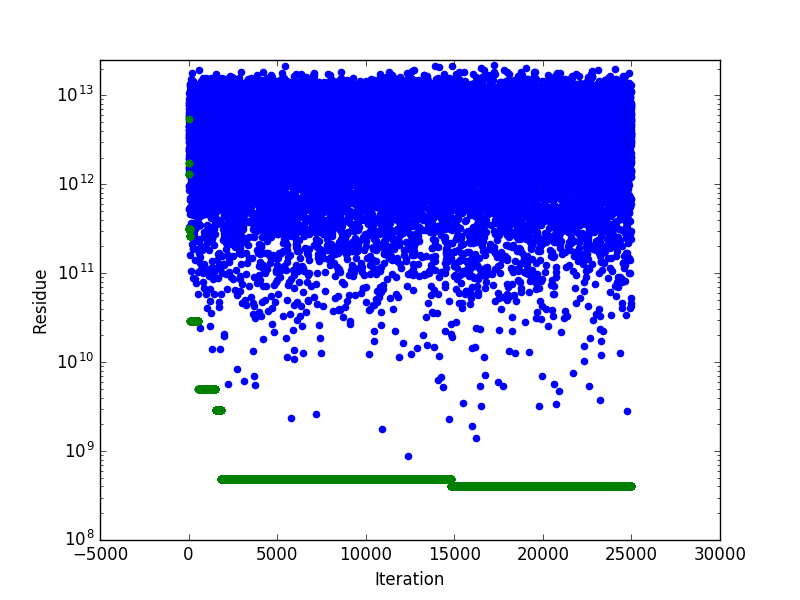
\includegraphics[width=\textwidth]{img/rrs.png}
\caption{RR (S)}
\end{subfigure}
\begin{subfigure}[t]{0.3\textwidth}
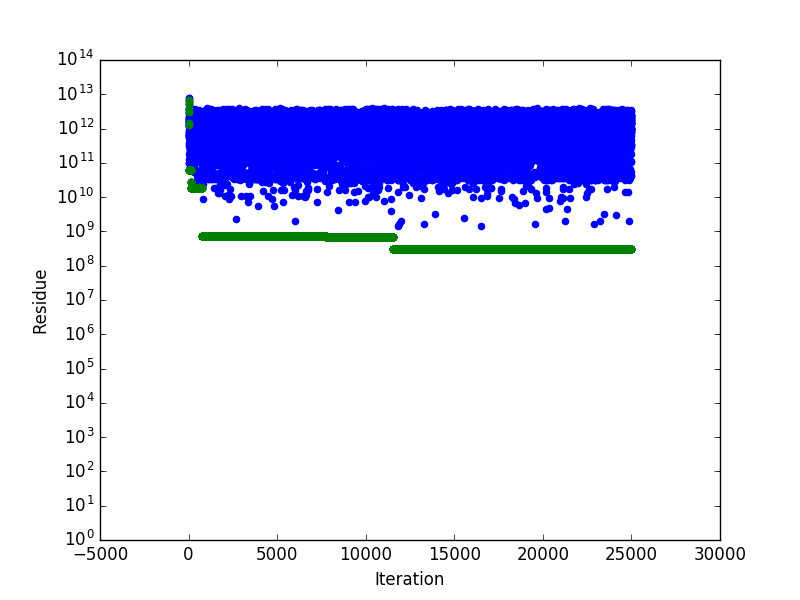
\includegraphics[width=\textwidth]{img/hcs.png}
\caption{HC (S)}
\end{subfigure}
\begin{subfigure}[t]{0.3\textwidth}
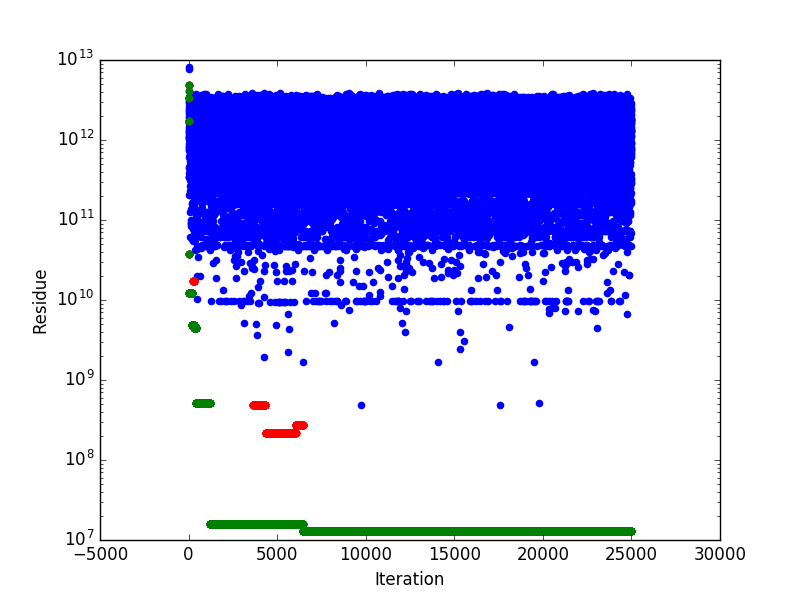
\includegraphics[width=\textwidth]{img/sas.png}
\caption{SA (S)}
\end{subfigure}\\
\begin{subfigure}[t]{0.3\textwidth}
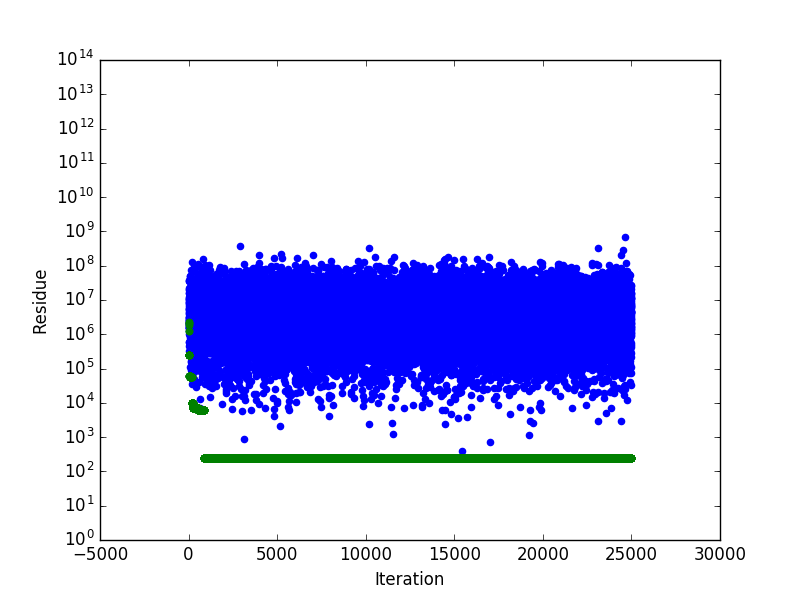
\includegraphics[width=\textwidth]{img/rrp.png}
\caption{RR (P)}
\end{subfigure}
\begin{subfigure}[t]{0.3\textwidth}
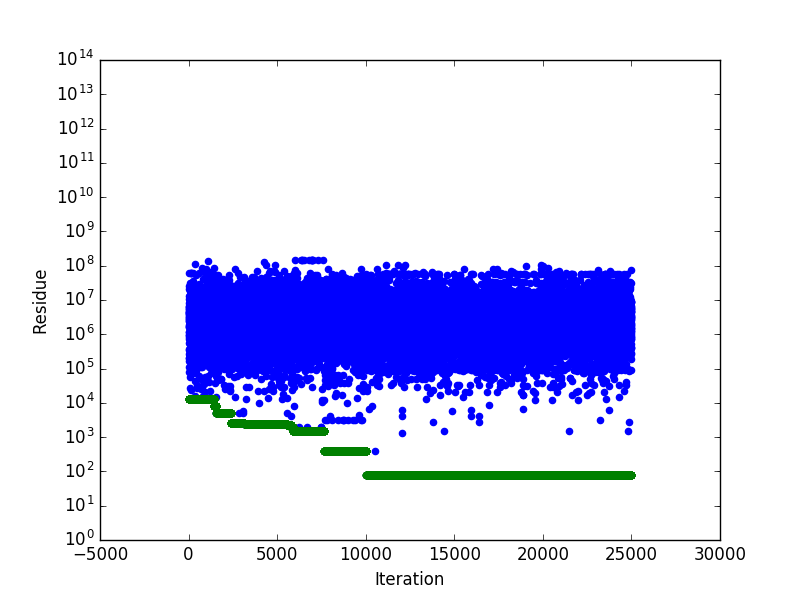
\includegraphics[width=\textwidth]{img/hcp.png}
\caption{HC (P)}
\end{subfigure}
\begin{subfigure}[t]{0.3\textwidth}
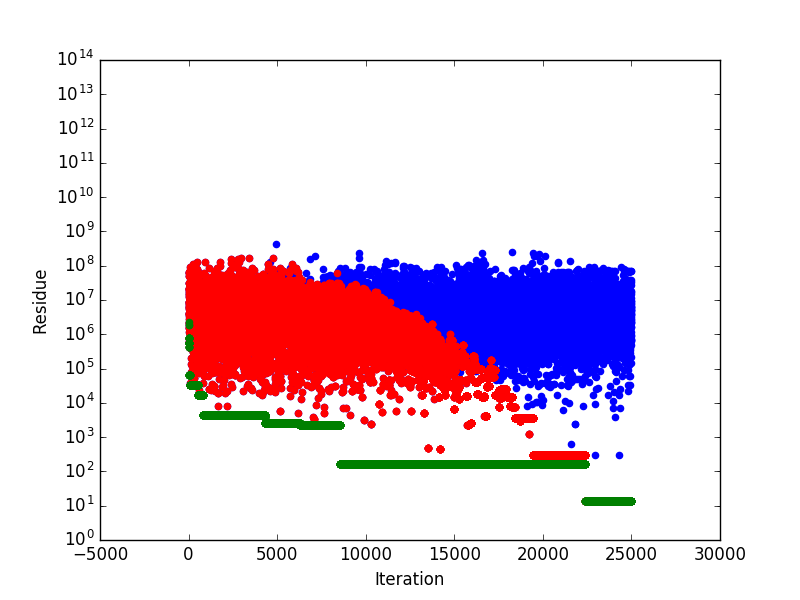
\includegraphics[width=\textwidth]{img/sap.png}
\caption{SA (P)}
\end{subfigure}
\caption{Residue Values During One Trial of Given Heuristic}
\end{center}
\end{figure}

We can draw a few conclusions from these graphs. First, the y-axis is on the same scale for all of them, so we can immediately see again that the prepartitioning produces better residues than the sequence. We also see that RR tends to fall to a minimum value early and stay there, which makes sense, since the probability of finding a lower residue by randomly selecting solutions decreases the lower our minimum residue is. We see a few more steps in HC, however. This occurs by nature of the fact that we only visit neighbors of a given solution. Thus we will not fall to a minimum quickly, but instead will gradually move toward the minimum over many iterations. SA for partition shows a gradual falling of the red dots. This corresponds to the cooling function making the algorithm less likely to choose poor solutions over time. This effect is not as obvious on the sequence graph, since the residue values are so high that the probability of shifting is almost zero. We can see that in both SA graphs, the best residue falls lower than the HC, since we allow for temporarily moving to worse neighbors in an attempt to find overall better ones. 

\section{Discussion}
Our goal was to implement various heuristics for the number partition problem, including the Karmarkar-Karp algorithm, as well as repeated random, hill climbing, and simulated annealing heuristics. We were able to do this, and our heuristics produced the results shown above. We have already discussed some of the conclusions we could draw from the results, but there are a few other thoughts we would like to touch on. \\

Above, we mentioned that prepartitioned solutions did better than sequence solutions, and we attributed this to the increased flexibility that prepartitioning provides. After all, the partitions we get are not themselves solutions; we still needed to run the KK algorithm on the partitions to produce a residue. Thus a fixed solution that would be given by a random sequence would be one possible solution to some prepartition, but the KK algorithm would likely find a more optimal solution that produces a lower residue. However, because the prepartition solution requires running the KK algorithm, we would expect some relationship between our prepartition results and our KK results. From figure 1, we can see that in general, the initial residue given a random preparition is higher than the residues produced by running the KK algorithm by itself, meaning random prepartitions perform worse than no prepartitions. This suggests that it may be more advantageous to just start the random heuristics with a one-to-one prepartitioning, as the initial residue would be exactly the KK residue. Over 25000 iterations, it may not matter for the final result, but we would on average have a lower starting point. \\

The fact that starting from the KK prepartition may be advantageous also suggests we should consider what happens if we start from the KK solution for the sequence-based heuristics. Again from figure 1, we see that most of the final residues from the sequence-based runs are higher than the KK residues. Thus starting with the KK solution will shift all of these down to at least the level of the KK solution. Whether the heuristics would then produce better results is debatable. The repeated random heuristic will likely not move the residues down much farther, since the probability of finding an even better solution randomly appears to be very small (based on where the band is currently). With the hill climbing heuristic, we expect that the results we have now suggest that we got stuck at local optima. Starting at a lower point should allow us to move to better solutions, though if the KK solution is a local optima itself, this will not happen. The simulated annealing heuristic may have the most opportunity to find a better final solution, since we'd start with a low enough residue that the probability of taking on a worse solution is higher than it was for our current trials. This would give the algorithm more flexibility in finding a lower optimal solution. \\

Thus overall, we would expect that starting with a KK solution instead of a random solution would mildly benefit our sequence heuristics, since we would have a much lower starting point. For the prepartitioned solutions, we would have a lower initial residue, but the overall benefit after 25000 iterations may not be as great, since we are already able to find solutions with very low residues. 



\pagebreak

\appendix
\section{Final Residues for Given Methods}
R: initial residue; RR: repeated random; HC: hill climbing; SA: simulated annealing \\\\
\begin{tabular}{c | c c c c | c c c c}
\multirow{2}{*}{KK}& \multicolumn{4}{c | }{Sequence} & \multicolumn{4}{c}{Partition} \\
& R & RR & HC & SA & R & RR & HC & SA \\ \hline
34971 & 10822420390057 & 155374873 & 95986951 & 376477989 & 40702703 & 233 & 413 & 89\\
10730 & 291879606832 & 228472382 & 320260752 & 167217288 & 4625566 & 136 & 14 & 304\\
167053 & 6673258379789 & 329663447 & 328624371 & 273723935 & 52648453 & 393 & 247 & 99\\
259754 & 1376845732664 & 313216286 & 36386704 & 158056782 & 473944 & 22 & 148 & 180\\
121504 & 7061089758030 & 772136136 & 317551920 & 105527580 & 1887368 & 468 & 618 & 150\\
51452 & 10343992443280 & 221317106 & 36503542 & 165552008 & 963940 & 270 & 1914 & 2\\
107573 & 4614462059233 & 85131791 & 464012333 & 772537577 & 808739 & 101 & 129 & 397\\
87981 & 1422808104157 & 25221665 & 501411629 & 530321089 & 67005061 & 63 & 83 & 235\\
13894 & 1356376628822 & 661091942 & 76203024 & 35073816 & 3324460 & 172 & 1710 & 146\\
92083 & 479177735597 & 921907615 & 77876597 & 193633973 & 2792567 & 41 & 723 & 371\\
138088 & 1249545622572 & 175909216 & 70245614 & 246420936 & 1941212 & 344 & 312 & 138\\
410883 & 243414920825 & 105658165 & 239796979 & 108474771 & 4646317 & 863 & 369 & 77\\
37706 & 11430392587090 & 39246218 & 120113616 & 446125528 & 38630924 & 144 & 6 & 474\\
4959 & 4067787093499 & 24759389 & 542265111 & 233971069 & 18963889 & 77 & 75 & 45\\
98982 & 2175280376182 & 100821554 & 1236938264 & 688213982 & 2188950 & 940 & 476 & 148\\
463510 & 1739069504278 & 139869568 & 75036270 & 11502710 & 175152 & 12 & 158 & 8\\
1644891 & 3495083184471 & 49560039 & 13720169 & 61430319 & 2537213 & 409 & 63 & 711\\
139281 & 351765857829 & 53398387 & 988468769 & 81428829 & 1802037 & 237 & 1005 & 381\\
394078 & 5755470980672 & 21353048 & 157391418 & 5971440 & 745400 & 186 & 630 & 36\\
107320 & 3895930206648 & 128708358 & 725491620 & 136598406 & 3992690 & 4 & 202 & 172\\
50804 & 12983588988310 & 451818596 & 99627184 & 118751320 & 1200558 & 4 & 2356 & 150\\
324855 & 5748524737771 & 325012143 & 223400605 & 452940573 & 1161801 & 75 & 105 & 699\\
135242 & 1728004920992 & 704083100 & 676644810 & 332982194 & 16588 & 164 & 754 & 276\\
145423 & 5441272197069 & 225423987 & 6201619 & 99470517 & 87319175 & 65 & 2927 & 367\\
123015 & 663595478753 & 528417633 & 1039183345 & 344036915 & 1417147 & 73 & 369 & 45\\
176602 & 6613491011748 & 294308518 & 273748166 & 688118388 & 18407516 & 294 & 1558 & 296\\
36304 & 1856766152536 & 161220750 & 455837768 & 83764346 & 26822008 & 1110 & 136 & 164\\
301760 & 1899256763434 & 113678664 & 585810298 & 243536474 & 1106016 & 202 & 204 & 0\\
63108 & 3427430057958 & 344589548 & 950945980 & 256413500 & 36730 & 146 & 0 & 794\\
360853 & 4036657978237 & 42220127 & 703414819 & 19806529 & 12418945 & 221 & 65 & 73\\
218412 & 900346511810 & 232196292 & 661249482 & 60944820 & 637880 & 164 & 608 & 14\\
3588550 & 2595831900490 & 1050246780 & 263865886 & 11475264 & 4786194 & 10 & 988 & 164\\
149598 & 1305294397646 & 187019180 & 111840076 & 240987176 & 2614908 & 308 & 14 & 8\\
\end{tabular}
\begin{tabular}{c | c c c c | c c c c}
\multirow{2}{*}{KK}& \multicolumn{4}{c | }{Sequence} & \multicolumn{4}{c}{Partition} \\
& R & RR & HC & SA & R & RR & HC & SA \\ \hline
407557 & 3926707064809 & 245517357 & 2022865 & 56030691 & 4436253 & 71 & 1959 & 1019\\
29832 & 1191540834240 & 19895442 & 174864454 & 443830502 & 7770892 & 14 & 4116 & 16\\
42600 & 3153800750690 & 293365844 & 355409068 & 681390488 & 557082 & 14 & 158 & 8\\
1601343 & 8202506007583 & 298681 & 200669301 & 185308965 & 4506947 & 103 & 221 & 373\\
23445 & 4971984587883 & 263411841 & 439607639 & 308089921 & 9394505 & 67 & 1169 & 247\\
233750 & 10790631655718 & 390750690 & 223805766 & 125872988 & 317398 & 478 & 162 & 12\\
49007 & 4536364976903 & 32133863 & 648138619 & 239303795 & 10757717 & 237 & 735 & 559\\
23680 & 6828193130916 & 104996518 & 39072626 & 200186108 & 32686 & 12 & 132 & 162\\
123578 & 4765629557230 & 156272448 & 54308150 & 57226240 & 13887404 & 188 & 1306 & 158\\
194223 & 1790585216809 & 183999215 & 880380253 & 335239229 & 13997805 & 221 & 693 & 71\\
793230 & 3283815385864 & 331839424 & 329715906 & 297449466 & 84776 & 804 & 930 & 40\\
158231 & 7046013476531 & 1036374145 & 30290799 & 135609771 & 84831 & 255 & 209 & 85\\
10258 & 8099798512072 & 24022596 & 382573088 & 103978728 & 678944 & 340 & 484 & 164\\
188740 & 564919194606 & 140730138 & 281475530 & 683221196 & 379688 & 16 & 2050 & 10\\
537599 & 7457286511807 & 23262437 & 306643805 & 346288531 & 206375 & 867 & 43 & 49\\
83636 & 375693290518 & 26821568 & 802226178 & 359693724 & 1832138 & 168 & 1704 & 16\\
39541 & 7750497829419 & 156552837 & 35869811 & 95481615 & 2787979 & 223 & 105 & 399\\
\end{tabular}

\pagebreak

\section{Runtimes for Given Methods}
RR: repeated random; HC: hill climbing; SA: simulated annealing \\
All runtimes in milliseconds \\\\
\begin{center}
\begin{tabular}{c c c | c c c c c c c c | c c c}
\multicolumn{3}{c | }{Sequence} & \multicolumn{3}{c}{Partition} & & & \multicolumn{3}{c | }{Sequence} & \multicolumn{3}{c}{Partition}\\
RR & HC & SA & RR & HC & SA & & & RR & HC & SA & RR & HC & SA \\ \cline{1-6} \cline{9-14}
47 & 16 & 19 & 1638 & 1576 & 1552 & & & 33 & 19 & 17 & 1648 & 1524 & 1581\\
39 & 18 & 20 & 1658 & 1518 & 1537 & & & 35 & 20 & 21 & 1637 & 1517 & 1504\\
38 & 20 & 19 & 1632 & 1467 & 1501 & & & 36 & 20 & 17 & 1644 & 1482 & 1500\\
36 & 25 & 20 & 1639 & 1520 & 1518 & & & 36 & 19 & 18 & 1621 & 1518 & 1504\\
39 & 29 & 17 & 1655 & 1525 & 1508 & & & 35 & 19 & 20 & 1632 & 1529 & 1515\\
44 & 21 & 17 & 1605 & 1544 & 1505 & & & 39 & 18 & 18 & 1610 & 1548 & 1484\\
41 & 17 & 17 & 1626 & 1555 & 1502 & & & 36 & 18 & 17 & 1655 & 1542 & 1493\\
40 & 18 & 20 & 1634 & 1561 & 1596 & & & 37 & 17 & 19 & 1647 & 1534 & 1572\\
38 & 18 & 20 & 1717 & 1505 & 1477 & & & 35 & 19 & 17 & 1635 & 1555 & 1475\\
44 & 19 & 17 & 1614 & 1523 & 1474 & & & 38 & 16 & 20 & 1662 & 1530 & 1577\\
38 & 19 & 20 & 1659 & 1541 & 1570 & & & 39 & 17 & 20 & 1663 & 1549 & 1530\\
34 & 17 & 18 & 1672 & 1550 & 1560 & & & 38 & 17 & 20 & 1633 & 1544 & 1573\\
37 & 19 & 21 & 1645 & 1470 & 1461 & & & 39 & 17 & 18 & 1678 & 1556 & 1569\\
34 & 18 & 17 & 1651 & 1516 & 1496 & & & 40 & 18 & 19 & 1627 & 1570 & 1492\\
36 & 19 & 20 & 1632 & 1576 & 1519 & & & 35 & 17 & 21 & 1667 & 1589 & 1512\\
42 & 18 & 17 & 1643 & 1508 & 1498 & & & 37 & 18 & 19 & 1639 & 1501 & 1544\\
44 & 17 & 19 & 1672 & 1568 & 1566 & & & 40 & 19 & 21 & 1647 & 1685 & 1588\\
36 & 17 & 17 & 1661 & 1548 & 1592 & & & 32 & 18 & 20 & 1648 & 1584 & 1572\\
36 & 17 & 18 & 1662 & 1584 & 1585 & & & 34 & 17 & 21 & 1642 & 1572 & 1605\\
36 & 20 & 20 & 1682 & 1575 & 1582 & & & 35 & 18 & 19 & 1717 & 1584 & 1590\\
37 & 19 & 23 & 1668 & 1559 & 1563 & & & 38 & 19 & 17 & 1679 & 1558 & 1609\\
36 & 17 & 19 & 1649 & 1546 & 1567 & & & 31 & 20 & 20 & 1670 & 1579 & 1578\\
37 & 19 & 18 & 1694 & 1583 & 1609 & & & 35 & 17 & 20 & 1681 & 1576 & 1612\\
32 & 20 & 25 & 1706 & 1625 & 1605 & & & 33 & 19 & 18 & 1683 & 1596 & 1567\\
31 & 17 & 22 & 1651 & 1622 & 1583 & & & 34 & 18 & 19 & 1698 & 1593 & 1569\\

\end{tabular}
\end{center}


\end{document}








